\begin{center}
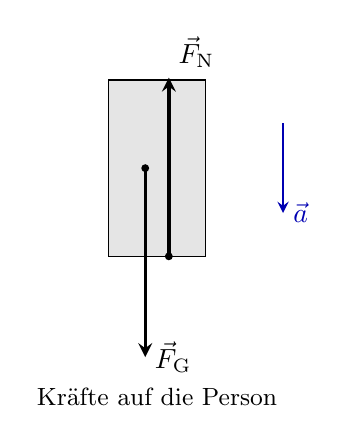
\begin{tikzpicture}[>=stealth]
 \draw[fill=gray!20] (-0.62,-1.12) rectangle (0.62,1.12);
 \draw[->, very thick] (-0.15,0) -- (-0.15,-2.4);
 \fill (-0.15,0) circle (0.05);
 \node[right] at (-0.15,-2.4) {$\vec F_\mathrm{G}$};
 \draw[->, very thick] (0.15,-1.12) -- (0.15,1.15);
 \fill (0.15,-1.12) circle (0.05);
 \node[above right] at (0.15,1.15) {$\vec F_\mathrm{N}$};
 \draw[->, thick, blue!70!black] (1.6,0.57) -- (1.6,-0.57) node[right] {$\vec a$};
 \node[font=\small] at (0,-2.9) {Kräfte auf die Person};
\end{tikzpicture}
\end{center}

\begin{abcliste}
\abc
Auf die Person wirken zwei Kräfte: die Gewichtskraft $\ssc{F}{G} = m\,g$ nach unten und die Kraft der Waage $\ssc{F}{N}$ (Normalkraft) nach oben. Der Lift wird nach unten schneller: Die Beschleunigung zeigt nach unten. Die resultierende Kraft zeigt in Richtung der Beschleunigung (Aktionsprinzip):
\begin{align}
 m\,g - \ssc{F}{N} &= m\,a
\end{align}
Also
\begin{align}
 \ssc{F}{N} &= \FNF \\
   &= \m\cdot(\g-\a) \\
   &= \FN \approx \result{\FNP{0}{3}}
\end{align}

\abc
Die Person drückt gleich stark auf die Waage (Wechselwirkungsprinzip), und die Waage teilt durch $g$:
\begin{align}
 \ssc{m}{W} &= \mAnF \\
   &= \frac{\FN}{\g} \\
   &= \mAn \approx \result{\mAnP{0}{3}}
\end{align}
Weniger als die Masse der Person: Sie fühlt sich leichter.
\end{abcliste}
